\documentclass{hcmutarticle}

\usepackage{amsmath}
\usepackage{multicol}
\setlength{\columnsep}{1cm}
% gói để tạo chữ giả, xóa đi khi viết báo cáo
%\usepackage{lipsum}

\usepackage{listings}
\usepackage{color}

\definecolor{dkgreen}{rgb}{0,0.6,0}
\definecolor{gray}{rgb}{0.5,0.5,0.5}
\definecolor{mauve}{rgb}{0.58,0,0.82}

\lstset{frame=tb,
	language=Java,
	aboveskip=3mm,
	belowskip=3mm,
	showstringspaces=false,
	columns=flexible,
	basicstyle={\small\ttfamily},
	numbers=none,
	numberstyle=\tiny\color{gray},
	keywordstyle=\color{blue},
	commentstyle=\color{dkgreen},
	stringstyle=\color{mauve},
	breaklines=true,
	breakatwhitespace=true,
	tabsize=3
}
% create the header for this file
\fancyhead[RO, LE]{\bf Bài toán khai báo tài liệu trích dẫn}

%\begin{center}
%	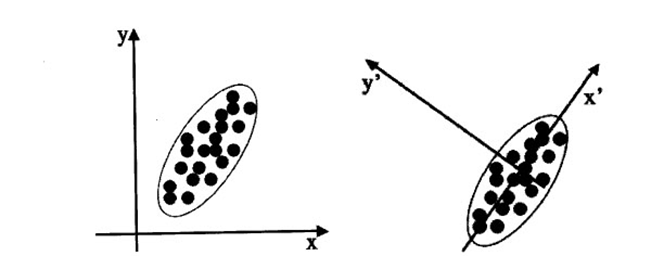
\includegraphics[scale=0.8]{image/figure.png}\\[0.5cm]
%	Figure 2.7: Two different sets of coordinate axes.The second consists of a rotation %and translation of the first and was found by using PCA.
%\end{center}

%\begin{itemize}
%	\item One entry in the list
%	\item Another entry in the list
%\end{itemize}
%\begin{enumerate}
%	\item The labels consists of sequential numbers.
%	\item The numbers starts at 1 with every call to the enumerate environment.
%\end{enumerate}
\begin{document}
\thispagestyle{empty}
\begin{center}
\LARGE\bfseries ĐẠI HỌC QUỐC GIA TP HỒ CHÍ MINH \\
TRƯỜNG ĐẠI HỌC BÁCH KHOA
\end{center}

\begin{center}

\includegraphics[scale=0.2]{hcmut.pdf}\\[1cm]
\end{center}

\vspace{1cm}

\begin{center}
\Large \bfseries BÁO CÁO BÀI TẬP LỚN MÔN NHẬN DIỆN MẪU VÀ HỌC MÁY\\[0.5cm]
\end{center}
\rule{\textwidth}{1pt}
\vspace{2pt}
\begin{center}
\Huge
\begin{tabular}{@{}l}
Study the PCA tool of WEKA \\
and apply it in feature extraction\\[6pt]
\end{tabular}
\end{center}
\rule{\textwidth}{1pt}\\[1cm]

\vspace{2cm}

\begin{minipage}[t]{0.60\linewidth}
\textbf{GVHD}: \\
\ PGS.TS. Dương Tuấn Anh
\end{minipage}
\begin{minipage}[t]{0.40\linewidth}
\textbf{Sinh viên thực hiện:}\\
Nguyễn Quốc Long - MSSV:1770023
\end{minipage}

\vspace{4cm}

\begin{center}

\textbf{TP.Hồ Chí Minh},
08/11/2018.

\end{center}



\newpage

\tableofcontents 

\newpage

\title{Bài luận tìm hiểu giải thuật Min-conficts}

\author{  Nguyễn Quốc Long\inst{1}} 

\institute{ MSSV: 1770023}




\maketitle



\begin{abstract}
Tài liệu tìm hiểu về giải thật PCA và phần mền WEKA.


\end{abstract}

\begin{keywords}
giảm chiều dữ liệu, giải thuật PCA, WEKA
\end{keywords} 


\section{Giới thiệu}

\textbf{Giảm chiều dữ liệu (Dimensionality Reduction)} 
 là một trong kỹ thuật quan trọng của Học Máy (Machine Learning). Các feature vectors trong các bài toán thực tế có thể có số chiều rất lớn, tới vài nghìn. Ngoài ra, số lượng các điểm dữ liệu cũng thường rất lớn. Nếu thực hiện lưu trữ và tính toán trực tiếp trên dữ liệu có số chiều cao này thì sẽ gặp khó khăn cả về việc lưu trữ và tốc độ tính toán. Vì vậy, giảm chiều dữ liệu sẽ làm tăng tốc độ tính toán nên đây là bước quan trọng trong nhiều bà toán học máy (đây cũng được gọi là phương pháp nén dữ liệu).
 
\textbf{Phân tích thành phần chính (Principal Component Analysis (PCA))}
 là một thuật toán Dimensionality Reduction dựa trên một mô hình tuyến tính. Phương pháp này dựa trên quan sát rằng dữ liệu thường không phân bố ngẫu nhiên trong không gian mà thường phân bố gần các đường/mặt đặc biệt nào đó. PCA xem xét một trường hợp đặc biệt khi các mặt đặc biệt có dạng tuyến tính là các không gian con (subspace).

\newpage

%%%%%%%%%%%%%%
\section{Giới thiệu công cụ Weka}\label{survey}
\textbf{Weka} (viết tắt của Waikato Environment for Knowledge Analysis) là một bộ phần mềm học máy được Đại học Waikato, New Zealand phát triển bằng Java. Weka là phần mềm tự do phát hành theo Giấy phép Công cộng GNU.

Để chạy chương trình, trước tiên người dùng cần tải Weka (64 bit) và tiến hành các thao tác cài đặt đơn giản. Sau khi hoàn tất quá trình cài đặt, Weka (64 bit) sẽ hiển thị bốn ứng dụng tích hợp cho phép người dùng truy cập, bao gồm "Explorer", "Experimenter", "KnowledgeFlow" và "Simple CLI".

Các tính năng chính của Weka (64 bit):

- Xem và phân tích tập tin dữ liệu ARFF.

- Thực hiện phân nhóm và hồi quy dữ liệu .

- Chỉnh sửa tùy thích hoặc lọc nội dung dữ liệu.

- Thay đổi thuộc tính và ảo hóa kết quả.

- Phân loại dữ liệu sẵn có theo quy tắc định trước.

- Tiến hành phân tích tổng lợi ích/chi phí.

- Lập biểu đồ dữ liệu.

- Khai thác kế hoạch Machine Learning.

- Lưu kết quả theo định dạng ARFF hoặc CSV hay cơ sở dữ liệu JDBC.

- Phân tích, kiểm thử tập tin dữ liệu.

%%%%%%%%%%%%%%
\section{Giới thiệu phương pháp PCA}\label{dev}
\textbf{PCA} là một thủ tục toán học biến đổi một số thuộc tính tương quan thành một số lượng nhỏ hơn các thuộc tính không tương quan được gọi là các thành phần chính. PCA là một phương pháp của Giảm chiều dữ liệu (Dimensionality reduction)

\textbf{Mục tiêu của PCA } là xác định cơ sở có ý nghĩa nhất để thể hiện lại một tập dữ liệu

\begin{center}
	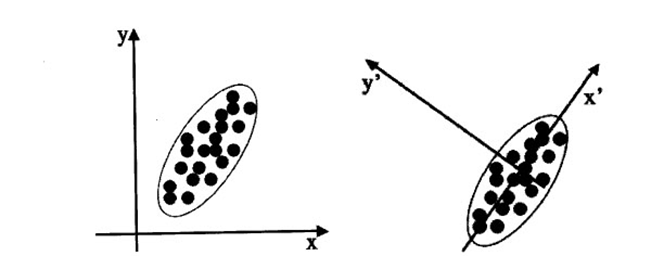
\includegraphics[scale=0.8]{image/figure.png}\\[0.5cm]
	Hình 2.7: Hình hai trục tọa độ khác nhau. Tọa độ thứ hai được quay và biến đổi từ tọa độ thứ nhất bằng cách sử dụng PCA
\end{center}
%Biến đổi ma trận \\
%\[
%\begin{bmatrix}
%x_{11}       & x_{12} & x_{13} & \dots & x_{1n} \\
%x_{21}       & x_{22} & x_{23} & \dots & x_{2n} \\
%\hdotsfor{5} \\
%x_{d1}       & x_{d2} & x_{d3} & \dots & x_{dn}
%\end{bmatrix}
%=
%\begin{bmatrix}
%x_{11} & x_{12} & x_{13} & \dots  & x_{1n} \\
%x_{21} & x_{22} & x_{23} & \dots  & x_{2n} \\
%\vdots & \vdots & \vdots & \ddots & \vdots \\
%x_{d1} & x_{d2} & x_{d3} & \dots  & x_{dn}
%\end{bmatrix}
%\]

\section{Các bước rút trích dữ liệu đặc trưng bằng phương pháp PCA trong công cụ Weka}

Các thông số có thể cấu hình cho giải thuật PCS của Weka \\

Tên class: weka.filters.unsupervised.attribute.PrincipalComponents.\\
Chương trình thực hiện phân tích thành phần chính và chuyển đổi dữ liệu.
Suy giảm số chiều được thực hiện bằng cách chọn đủ các hàm riêng để chiếm một số phần trăm phương sai trong dữ liệu gốc - mặc định giá trị này là 0.95 (95%)
Chương trình dựa vào code lựa chọn thuộc tính 'PrincipalComponents' của hai tác giả  Mark Hall và Gabi Schmidberger.

\begin{enumerate}
	\item centerData -- Tìm điểm trung tâm của dữ liệu (thay vì chuẩn hóa). PCA sẽ được tính toán từ ma trận hiệp phương sai (chứ không phải từ khoảng cách tương quan)
	\item debug -- Nếu được đặt thành true, bộ lọc có thể xuất thông tin bổ sung cho console
	\item varianceConvered -- Giữ lại đủ các thuộc tính PC dể chiếm tỉ lệ phương sai này
	\item maximumAttribution -- Số lượng thuộc tính PC tối đa được giữ lại
	\item maximumAttributeNames  -- Số lượng thuộc tính tối đa bao giồn trong tên thuộc tính được chuyển đổi
	\item doNotCheckCapabilities  -- Nếu được đặt giá trị, khả năng của bộ lọc sẽ không được kiểm tra trước khi nó được xây dựng. (Sử dụng thận trọng để giảm thời gian chạy)
\end{enumerate}
\begin{multicols}{2}
	[
	Dữ liệu đầu vào cho chương trình WEKA
	]
	\begin{lstlisting}
	% 1. Title: PCA Database
	% 
	% 2. Sources:
	%      (a) Creator: nqlong
	%      (c) Date: Jan, 2019
	% 
	@RELATION iris
	
	@ATTRIBUTE x  NUMERIC
	@ATTRIBUTE y  NUMERIC
	@ATTRIBUTE class        {1,2}
	
	@data
	1,1,1
	1,2,1
	1,3,1
	2,1,1
	2,2,1
	2,3,1
	2,3.5,1
	2.5,2,1
	3.5,1,1
	3.5,2,1
	3.5,3,2
	3.5,4,2
	4.5,1,2
	4.5,2,2
	4.5,3,2
	5,4,2
	5,5,2
	6,3,2
	6,4,2
	6,5,2
	\end{lstlisting}
	
	\begin{center}
		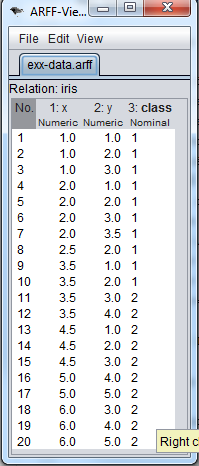
\includegraphics[scale=0.4]{image/data_weka.png}\\[0.5cm]
		Hình 3: Dữ liệu đầu vào cho giải thuật PCA của Weka
	\end{center}
\end{multicols}



Tiếp theo, ta thiết lập cấu hình cho phần mềm WEKA
\begin{center}
	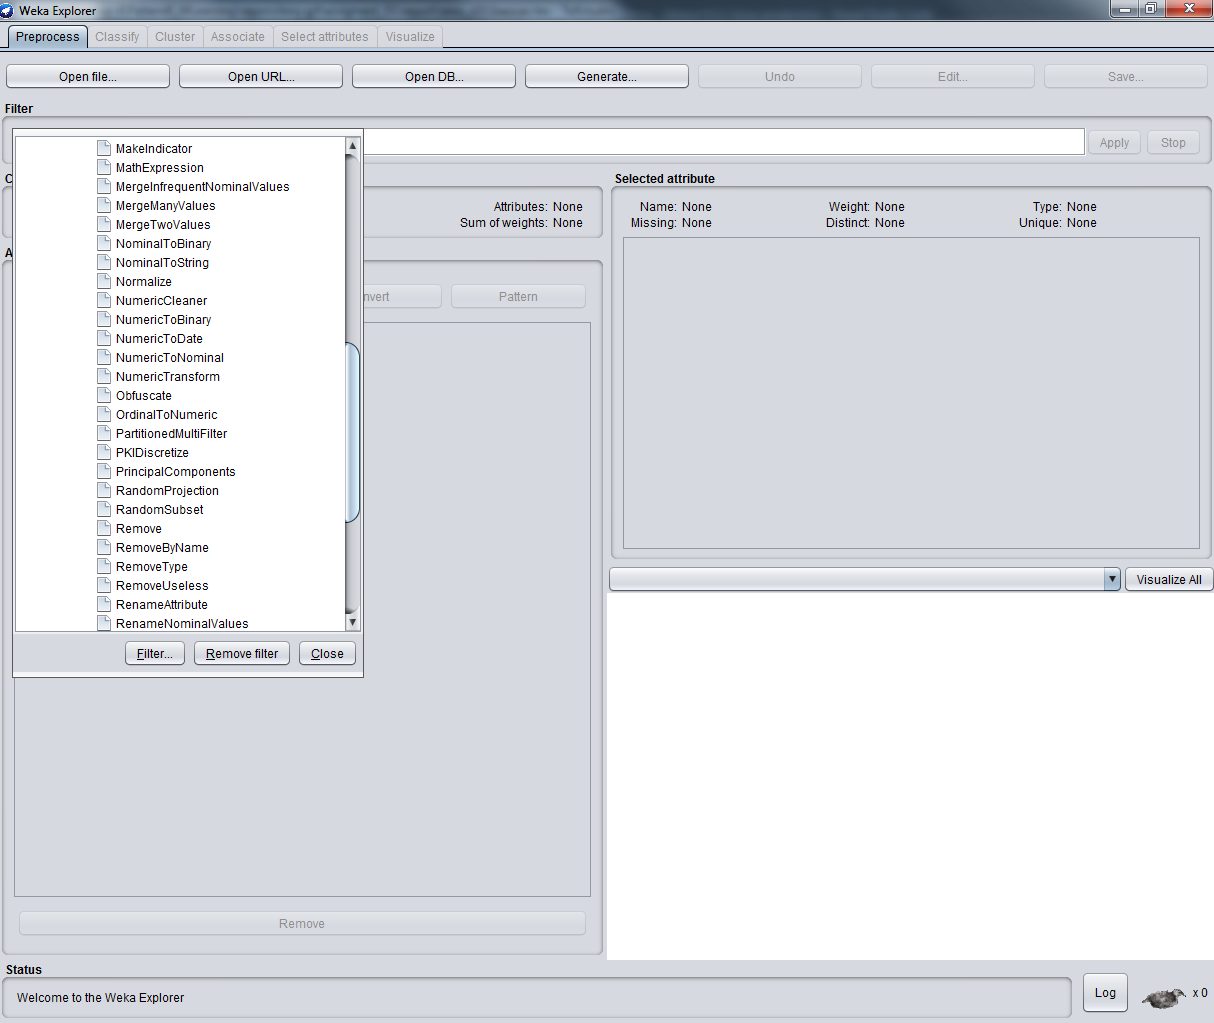
\includegraphics[scale=0.4]{image/step1.png}\\[0.5cm]
	Hình 4: Lựa chọn giải thuật PCA 
\end{center}
% pca_1.png
% result_1.png
Tiếp theo sau đó, ta tải dữ liệu vào phần mềm Weka và áp dụng giải thuật PCA của Weka để tìm ra kết quả
\begin{center}
	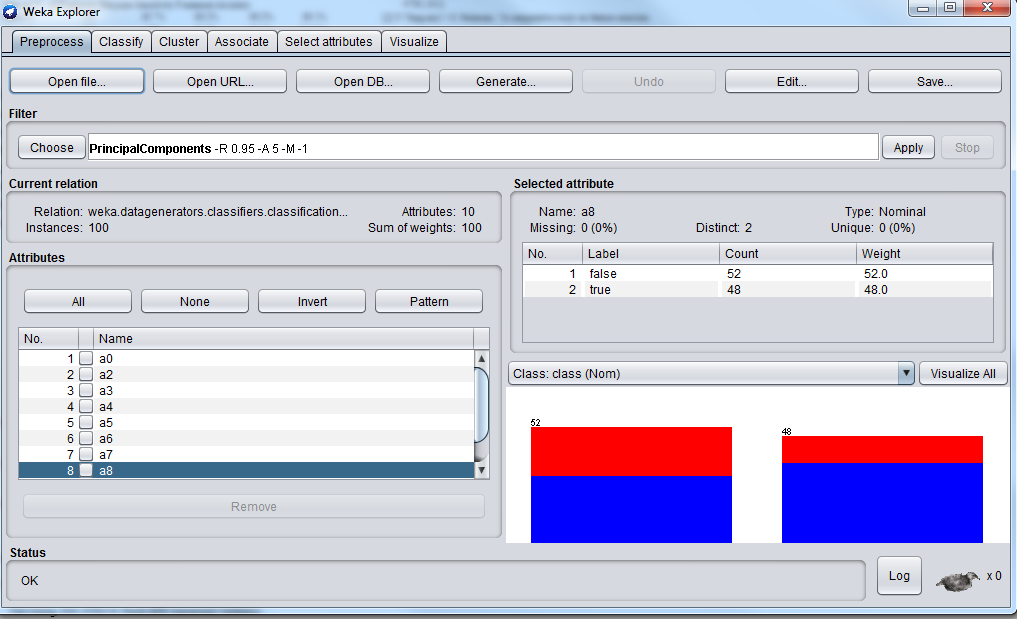
\includegraphics[scale=0.5]{image/pca_1.png}\\[0.5cm]
	Hình 5: Kết quả load dữ liệu mẫu
\end{center}

\begin{center}
	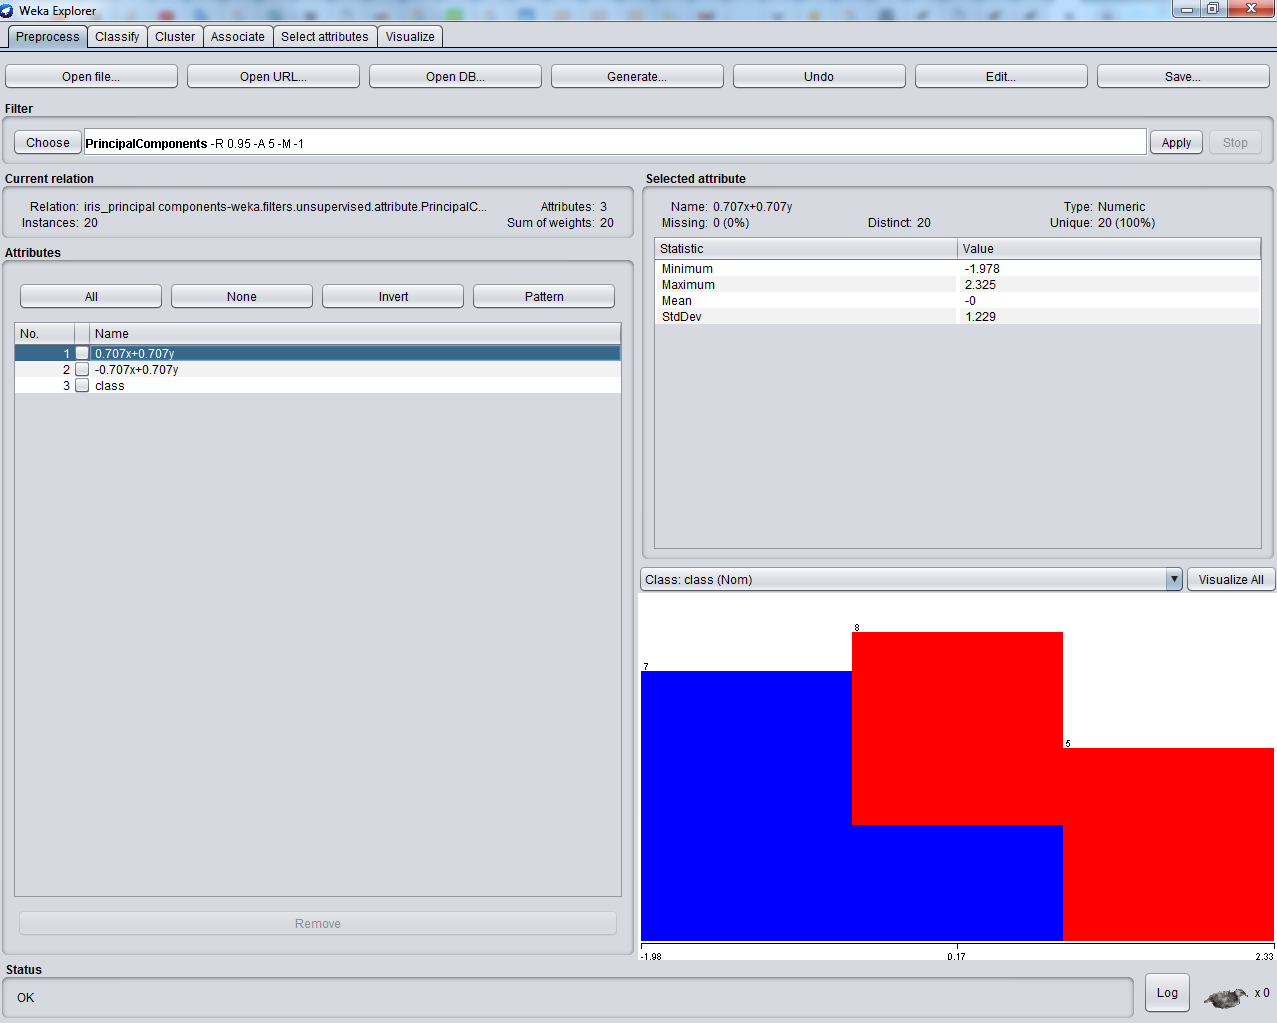
\includegraphics[scale=0.4]{image/result_1.png}\\[0.5cm]
	Hình 6: Kết quả của việc áp dụng giải thuật PCA (1)
\end{center}

\begin{center}
	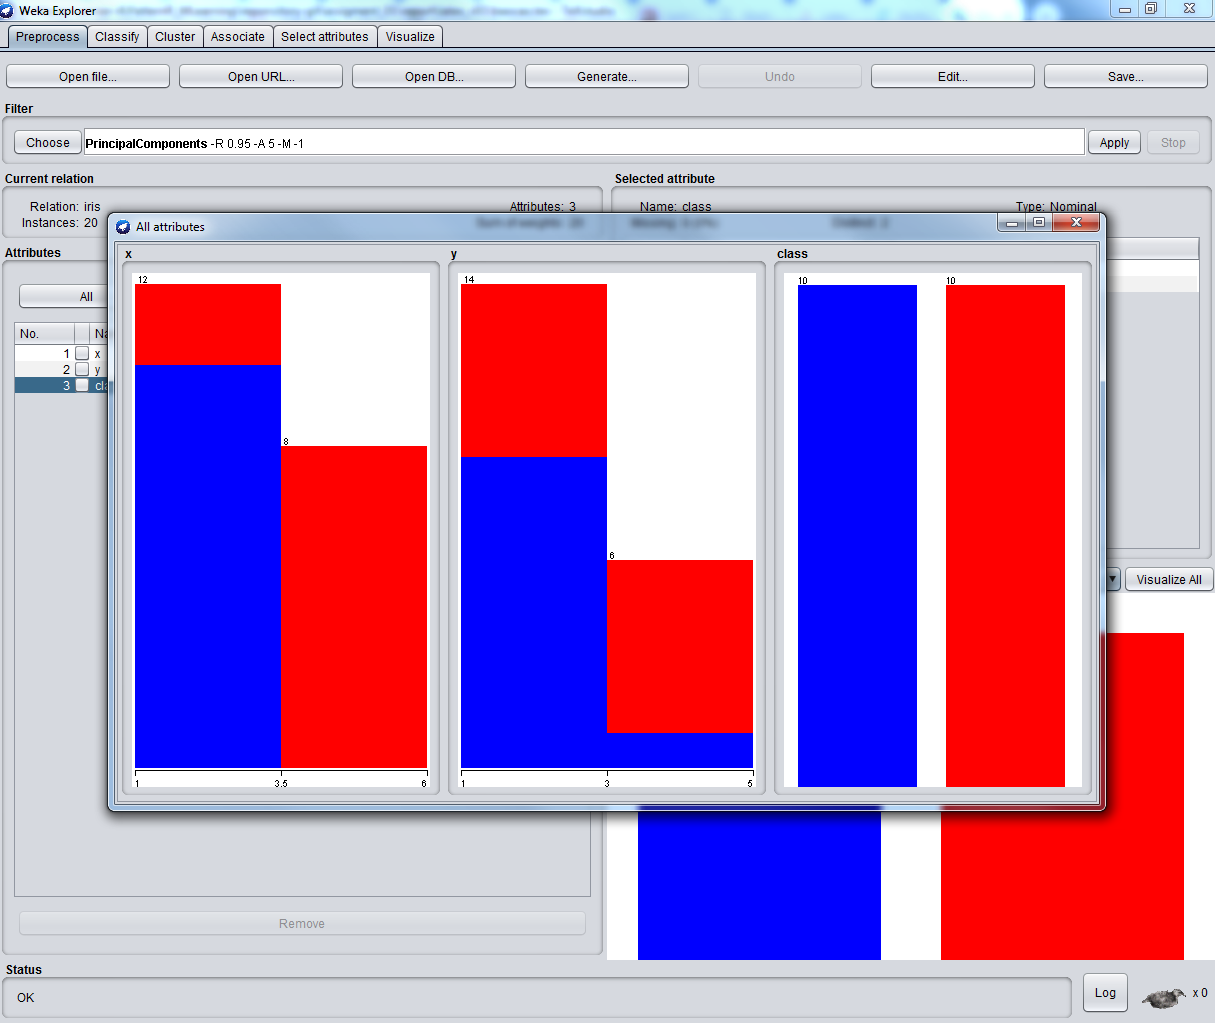
\includegraphics[scale=0.4]{image/resultAll.png}\\[0.5cm]
	Hình 7: Kết quả của việc áp dụng giải thuật PCA (2)
\end{center}

%%%%%%%%%%%%%%
\section{Kết Luận }\label{result}
Tài liệu được thực hiện  với sự giúp đỡ tận tình của giáo viên hướng dẫn, Thầy TS. Dương Tuấn Anh\\
Trong quá trình nghiên cứu, thực hiện không thể tránh khỏi những  thiếu sót, kính mong quý thầy  cô và các bạn đóng góp thêm để tài liệu thêm hoàn thiện.\\
Xin chân thành cảm ơn.


%%%%%%%%%%%%%%
\section{Tài liệu Tham Khảo }




%%%%%%%%%%%%%%%%%%%%%%%%%%%%%%%%%
%https://vi.wikipedia.org/wiki/Weka_(h%E1%BB%8Dc_m%C3%A1y)
http://en.wikipedia.org\\
https://machinelearningcoban.com/2017/06/15/pca/ \\
%https://waikato.github.io/weka-wiki/arff_stable/

%%%%%%%%%%%%%%

\end{document}



